\documentclass[12pt]{article}
\usepackage{amsmath}
\usepackage{amssymb} %mathbb
\usepackage{graphicx}
\usepackage{hyperref}
\usepackage{xcolor}
\usepackage{gensymb}
\usepackage[latin1]{inputenc}
\usepackage[top=1.0cm,bottom=1.3cm,left=1.0cm,right=1.0cm]{geometry}

\begin{document}

\Large

\begin{center}
  Projeto Intervalar
\end{center}

\vspace{3mm}

\normalsize

N\~ao gosto de MatLab por nunca ter visto um execut\'avel. A primeira linguagem de programa\c{c}\~ao foi Delphi. Mas houve barreira de plataforma: do meu lado Windows, do lado do orientador iMac. Por isto, escolhi a linguagem Java: roda em qualquer lugar. No semestre 2018/1, eu j\'a tinha um projeto de Enciclop\'edia Esp\'irita em java, que fazia pesquisa e cadastro em banco de dados. Tabelas de verbetes, de postagens, de categorias, de usu\'arios, de anexos (blob), de idiomas, de vota\c{c}\~ao. Ele evoluiu para c\'alculo de polin\^omios de milh\~oes de termos em banco de dados. No semestre 2019/2, eu estava matriculado em Reconhecimento de Padr\~oes, e preparei um projeto Classificador de Bayes. Dividi meu Giant Hello World em github.com/boralaemcasa/wiki.git com banco de dados e github.com/boralaemcasa/spiritistwiki.git sem nenhum banco de dados. No semestre 2020/1, iniciamos este projeto intervalar j\'a com esqueleto copiado, temos dispon\'ivel para utilizar (apesar de estar extremamente lento) o tratamento de fra\c{c}\~oes em tipo String, com numerador e denominador de bilh\~oes de d\'igitos (ou os teraBytes que estiverem dispon\'iveis).

Temos fontes no reposit\'orio github. Quando eu rodo git push, o site heroku.com l\^e os fontes, compila e faz deploy para http://spiritistwiki.herokuapp.com . Estou utilizando html, css, javascript, ajax, worker, spring boot, maven, thymeLeaf, jquery datatables (https://cdn.datatables.net/1.10.19/), codifica\c{c}\~ao UTF-8.

O servidor faz 99\% do processamento com Apache e TomCat. O usu\'ario entra na raiz do site (index.html), de qualquer sistema operacional com camada de browser. Nem de m\'aquina virtual JVM instalada ele precisa. Eu exijo que o javascript n\~ao esteja bloqueado. H\'a quatro coisas na raiz: anexos do facebook, meus opus, meus tEx, link para idioma portugu\^es e idioma ingl\^es (para futura tradu\c{c}\~ao).

O usu\'ario seleciona Portugu\^es (principal.html). As $3$ primeiras linhas s\~ao compatibilidade com o projeto wiki.git. Abaixo h\'a op\c{c}\~oes de:

(1) Fuzzy Intervalar;

(2) Classificador Bayes;

(3) somar duas fra\c{c}\~oes: $a/b + c/d$;

(4) $a/b - c/d$;

(5) $a/b \times c/d$;

(6) $a/b / (c/d)$;

(7) Pot\^encia: $a/b \wedge c/d$;

(8) Bin\^omio de Newton: $(n, p) = (a/b, c/d)$;

(9) Comandos: (o mais complicado testado resolve ax + b = c);

(10) Calcular Gamma($a/b$), pela integral, dado o valor de $ds = c/d$;

(11) Floor($a/b$);

(12) Exponencial($a/b$), pela s\'erie de Taylor, dado o valor do erro $< c/d$;

(13) Pot\^encia: $\exp(c/d \ln (b/a))$, pela s\'erie de Taylor, dado o valor do erro $< c/d$;

(14) Log de $a/b$ na base $c/d$, pela s\'erie de Taylor, dado o valor do erro $< e/f$;

(15) $\ln (a/b)$, pela s\'erie de Taylor, dado o valor do erro $< c/d$;

(16) N\'umeros de CarMichael m\'odulo $m \ge 3$.

(17) Resolver a equa\c{c}\~ao diofantina $ax + by = 1$.

(18) mdc de dois inteiros;

(19) mmc de dois inteiros;

(20) ordem um inteiro m\'odulo $m \ge 3$.

(21) ordena\c{c}\~ao de $\mathbb{Z}^2$ por espiral. Op\c{c}\~ao de fra\c{c}\~ao $p/q$ com termos primos entre si. Op\c{c}\~ao de semiplanos.

O usu\'ario clica no bot\~ao Fuzzy Intervalar (fuzzy\_pt.html). RequestMapping("/fuzzy\_pt/abrir"). Inicializa uma sess\~ao de usu\'ario.

Na coluna da esquerda eu preparei entrada e sa\'ida do tipo Double. PostMapping("/fuzzy\_pt/selecionar1")

Na coluna da direita eu preparei entrada e sa\'ida da classe Interval. PostMapping("/fuzzy\_pt/selecionar2") Um intervalo tem um m\'inimo e um m\'aximo. Implementei constantes $\pm$ infinity = $\pm 1.75e308$.

\vspace{100mm}

O ambiente est\'a preparado para ao clicar em um bot\~ao, dar in\'icio ao uma thread demorada. Se eu n\~ao fizesse isso, eu deveria responder imediatamente ao browser em tempo m\'aximo de $30$ segundos. Depois que eu fiz isso, o limite passa para $30$ minutos, pois se passar disso o heroku.com faz undeploy da aplica\c{c}\~ao por inani\c{c}\~ao. Entendemos que dependendo do loop infinito que estiver rodando h\'a meia hora, isso deve custar caro ao processador do servidor no exterior. (Eu acho que \'e europeu. O hor\'ario do servidor \'e GMT.)

\`A medida que a thread roda, ela emula um println no browser do usu\'ario. O worker de segundo em segundo chama o GetMapping("/fuzzy\_concluido") at\'e que retorne ``Processamento conclu\'ido". A thread tem uma vari\'avel private String saida1, que de um momento a outro publica em sess\~ao via session.setAttribute(attr, saida1.replace(``$\setminus$n", ``$\langle br/\rangle$")). Outro GetMapping, no mesmo timing do worker, compartilha da sess\~ao com o usu\'ario.

Antes de clicar em Fuzzy Double, h\'a algumas possibilidades de entrada.txt (via textArea ou memorando). A primeira palavra \'e o comando:

(1) square $x_1$ $x_2$ retorna quadrado de um intervalo. O que importa \'e se entre as entradas h\'a uma \'unica barra de espa\c{c}o ou ``$\setminus$n". E tem que ter um caracter desses no final. Texto sobrando \'e ignorado.

(2) exp $x_1$ $x_2$ retorna exponencial de um intervalo.

(3) plus $x_1$ $x_2$ $y_1$ $y_2$ retorna soma de dois intervalos.

(4) minus $x_1$ $x_2$ $y_1$ $y_2$ retorna intervalo menos intervalo.

(5) times $x_1$ $x_2$ $y_1$ $y_2$ retorna produto de dois intervalos.

(6) over $x_1$ $x_2$ $y_1$ $y_2$ retorna intervalo dividido por intervalo.

(7) equals $x_1$ $x_2$ $y_1$ $y_2$ retorna verdadeiro ou falso, se intervalo = intervalo.

(8) lessthan $x_1$ $x_2$ $y_1$ $y_2$ retorna verdadeiro ou falso, se intervalo $<$ intervalo.

(9) le $x_1$ $x_2$ $y_1$ $y_2$ retorna verdadeiro ou falso, se intervalo $\le$ intervalo.

(10) gauss $x_1$ $x_2$ $c_1$ $c_2$ $\sigma_1$ $\sigma_2$ retorna a f\'ormula da gaussiana: $y = e^{-0.5 \cdot (c-x)^2/\sigma^2}$.

\begin{verbatim}
	public Interval gauss(Interval c, Interval sigma) {
	..Interval temp1 = c.minus(this); // onde this � nosso x.
	..temp1 = temp1.over(sigma);
	..Interval temp2 = temp1.square();
	..temp1 = temp2.timesConstant(-0.5);
	..return temp1.exponential();
	}
\end{verbatim}

(11) else. No caso geral, as entradas necess\'arias a seguir s\~ao: xleft xright ybottom ytop alfa nGaussianas nVari\'aveis n\'Epocas xi\_t xf\_t step\_t xi\_v xf\_v step\_v.

Por exemplo, suponhamos que os limites do gr\'afico s\~ao -6.4 6.4 -1.4 1.4; alfa = 0.001; 5 gaussianas; 1 vari\'avel; 500 \'epocas; -6.3 6.3 0.1 de treinamento; -6.25 6.25 0.1 de valida\c{c}\~ao.

Outro exemplo do livro tem 3 vari\'aveis; 1 6 1 de treinamento; 1.5 5.5 1 de valida\c{c}\~ao.

Mas qual \'e a fun\c{c}\~ao $y = f(x_1, x_2, x_3)$? No caso do intervalo, inicialmente $[y] = \sin [x]$, e na vers\~ao atual est\'a a norma da soma. $y = |x_1| + \cdots + |x_n|$.

(12) caso o comando seja livro, e o n\'umero de vari\'aveis seja 3, a f\'ormula est\'a fixa em $y = 1 + \sqrt{x_1} + \cfrac{1}{x_2} + \cfrac{\sqrt{x_3}}{x_3}$.

(13) caso o comando seja lista, as entradas necess\'arias a seguir s\~ao: xleft xright ybottom ytop alfa nGaussianas nVari\'aveis n\'Epocas nPontosT nPontosV xt(i) ydt(i) xv(i) ydv(i).

Desta forma emulamos o exemplo do livro sobre equa\c{c}\~ao do caos, ponto a ponto.

\vspace{3mm}

Terminada a introdu\c{c}\~ao, o que faz o fuzzy afinal? Quem como eu fez a disciplina Sistemas Nebulosos sabe.

Primeiro monte as matrizes e vetores $(x,y)$ abaixo.

			xt = new Double[nPontosT][nVari\'aveis];

			xv = new Double[nPontosV][nVari\'aveis];

			ydt = new Double[nPontosT];

			ydv = new Double[nPontosV];

Segundo, rode o fuzzy 8 vezes, para o mesmo alfa, para tr\^es par\^ametros true ou false. Chamei isso de calcularAPE. Retorna a seguinte classe:

\begin{verbatim}
public class AverageError {
..public SaidaDouble saidaDouble;
..public Integer epocas;
..public Double ape;
..public Double alpha;
..Double[] q;
..Double[][] p;
..Double[][] c;
..Double[][] sigma;
}
public class SaidaDouble {
..public Double [] ys;
..public Double [] omega;
..public Double [] z; // aquele y_i que tem no meio das formulas troquei por z
..public Double denom;
}
..for (i = 0; i < 32; i++, alpha += 1e-6)
....erro[i] = calcularAPE(alpha, nEpocas, nPontosT, nPontosV, xt, xv, ydt, ydv,
......nVariaveis, nGaussianas, xit,	xft);
\end{verbatim}

Cada c\'alculo desses se resume em:

(1) inicializar $p$ com matriz aleat\'oria; inicializar $q$ com vetor aleat\'orio;

(2) inicializar $c$ com valores igualmente distanciados;

(3) toda a matriz $\sigma$ \'e inicialmente constante e igual a $0.5 \cdot (x_{ft} - x_{it}) / (\text{nGaussianas} - 1) / \sqrt{2 \cdot \ln 2}$;

(4) para cada (\'epoca, ponto de treinamento) fa\c{c}a:

(4.1) calcule a sa\'ida de um ponto de treinamento;

Retorna $\omega_j = \Pi_j \text{gauss}(c[j][v], \sigma[j][v]) $, onde $j$ varia com o n\'umero de gaussianas

e $v$ com o n\'umero de vari\'aveis;

Retorna $z_j = q_j + \sum_j p[j][v] \cdot X[k][v]$, onde $k$ varia com o n\'umero de pontos, que aqui \'e igual a $1$;

N\~ao retorna ysd$_k = \sum_j \omega_j$, mas retorna somente denom = ysd$_0$;

Retorna $\text{ys}_k =  1 / \text{ysd}_k \cdot \sum_j (\omega_j \cdot z_j)$.

(4.2) para cada (gaussiana, vari\'avel), fa\c{c}a:

(4.2.1) calcule o gradiente do erro em rela\c{c}\~ao ao vetor $v = (c, \sigma, p, q)$;

$\cfrac{\partial e}{\partial c[j][v]} = $ dedys $\cdot$ dysd$\omega$j $\cdot$ d$\omega$jdcij, onde dedys = ys$[0] -$ ydt[k];

$\cfrac{\partial e}{\partial \sigma[j][v]} = $ dedys $\cdot$ dysd$\omega$j $\cdot$ d$\omega$jdsij, onde dysd$\omega$j = ($z_j - $ys[0]) / denom;

$\cfrac{\partial e}{\partial p[j][v]} = $ dedys $\cdot$ dysdyj $\cdot$ dyjdpij, onde d$\omega$jdcij $= \omega[j] \cdot$ difx / $\sigma_j^2$;

$\cfrac{\partial e}{\partial q_j} = $ dedys $\cdot$ dysdyj, onde d$\omega$jdsij $= \omega_j \cdot$ difx / $\sigma_j^3$;

onde dysdyj $= \omega_j$; onde dyjdpij $= x_t[k][v]$; e onde difx $= (x_t[k][v] - c[j][v])^2$.

(4.2.2) ajuste $v = v - \alpha \cdot \nabla e$;

(5) calcule a sa\'ida de todos os pontos do vetor de valida\c{c}\~ao;

(6) calcule o erro percentual m\'edio (APE) = $\sum_k \vert \text{ys}[k] - \text{ydv}[k]\vert / \vert \text{ys}[k] \vert \cdot 100 /$ nPontosV.

Quando tiver na mem\'oria $8$ males, dos males o menor erro.

\vspace{3mm}

Explicando os par\^ametros booleanos calcularAPE(normalizar, limitar, copiar).

if (normalizar) dedys /= Math.abs(dedys); // ao depurar, eu vi esse m\'odulo ir para infinito.

if (limitar \&\& (max $>$ 100.0))	alpha *= 0.01; // onde max \'e a norma do m\'aximo do $\nabla e$, que de vez em quando estava gigante.

if (copiar) \{

..1) calcule a sa\'ida de todos os pontos do vetor de valida\c{c}\~ao;

..2) calcule o erro percentual m\'edio (APE);

..3) se o valor encontrado for maior que zero e menor que o m\'inimo (ou se for o primeiro), copie-o para o Result := m\'inimo.

\}

O efeito desse copiar \'e que se voc\^e pedir $100$ \'epocas, algumas vezes o programa p\'ara em $95$ \'epocas, a $96^a$ \'epoca tem APE maior que o m\'inimo.

\vspace{3mm}

A fim de que o usu\'ario visualize, vamos plotar o melhor gr\'afico com $y_v$ em azul, e sa\'ida em vermelho.

\begin{verbatim}
		if (nVariaveis > 1) {
		..xleft = -1.0;
		..xright = 1.0 + (double) nPontosV;
		}
\end{verbatim}

Se for uma vari\'avel, plote $(x,y_v)$, caso contr\'ario, plote $(i, y_v)$, com i variando de zero ao nPontosV.

\vspace{3mm}

Primeiro movimento: implementei o intervalo do livro e o erro estava muito grande, chegando a infinito em dez \'epocas.

Desconfiei de fun\c{c}\~oes decrescentes invertendo o m\'aximo e o m\'inimo do intervalo. Desconfiei do quadrado. Desconfiei do cubo. Desconfiei da gaussiana. Nada deu certo.

\vspace{3mm}

Segundo movimento: troquei o intervalo do livro por vetor de dez pontos. Quando consegui erro baixo para par\'abola, fiz todos os testes novamente. Os resultados seguem apresentados abaixo.

\vspace{3mm}

Terceiro movimento: retroalimenta\c{c}\~ao. Se o comando for igual a lista, vamos retroalimentar nRetro vezes.

Retro 1:

\vspace{3mm}

obj averageInterval := averageError;

ixv := xv;

obj.calcularSaidaInterval(ixv);

\vspace{3mm}

Retro $2, 3, \cdots,$ nRetro:

\vspace{3mm}

for (v = 1; v $<$ nVariaveis; v++) ixv[j][v].set(ixv[j][v - 1]); // shift right

ixv[j][0].set(obj.saida.ys[j]);  // manda da sa\'ida para a coluna zero da entrada

obj.calcularSaidaInterval(ixv);

\vspace{200mm}

Teste 1 | Caso Geral | Uma vari\'avel

curva

-6.4 6.4 -0.1 6.5

0.01

5 1 500

-6 6 0.1

-5.5 5.5 0.1

Average Error 1.870942855116726\%

alfa = 0.010007999999999994

Gr\'afico:

		\begin{center}
		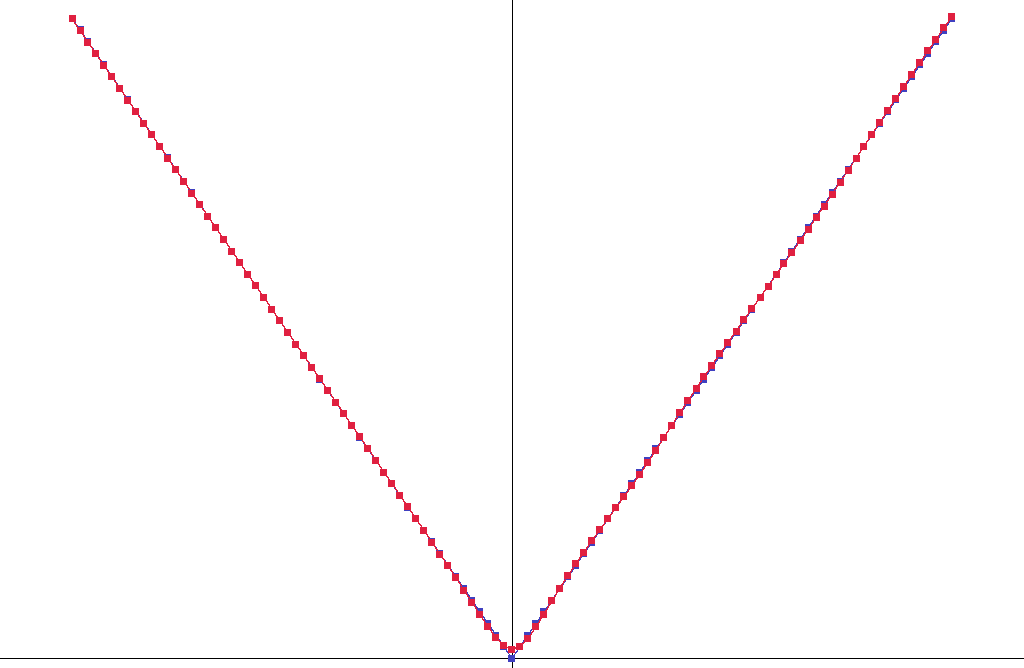
\includegraphics[scale=0.7]{uma_variavel}
		\end{center}

\vspace{100mm}

Teste 2 | Caso Geral | Duas vari\'aveis

curva

-6.4 6.4 -0.1 12.5

0.01

5 2 500

-6 6 1

-5.5 5.5 1

Average Error 1.7216122112761425\%

alfa = 0.010003999999999997

Gr\'afico:

		\begin{center}
		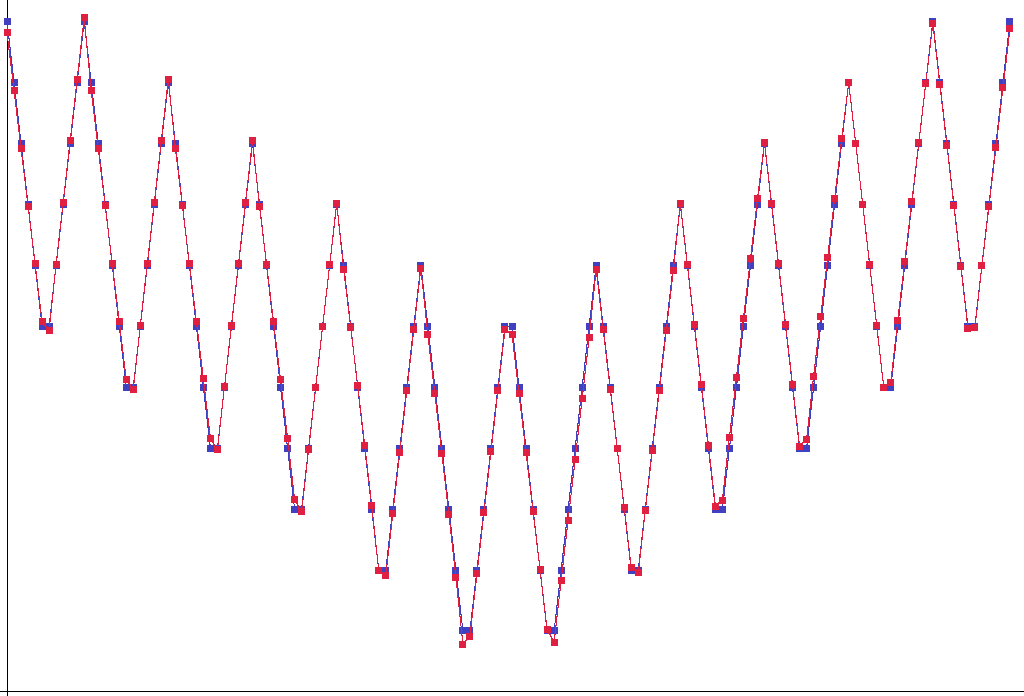
\includegraphics[scale=0.7]{duas_variaveis}
		\end{center}

\vspace{100mm}

Teste 3 | Comando livro | Tr\^es vari\'aveis

livro

-1 126 -0.1 6

0.0002

3 3 500

1 6 1

1.5 5.5 1

Average Error 3.5211582845088265\%

alfa = 2.2899999999999993E-4

Gr\'afico:

		\begin{center}
		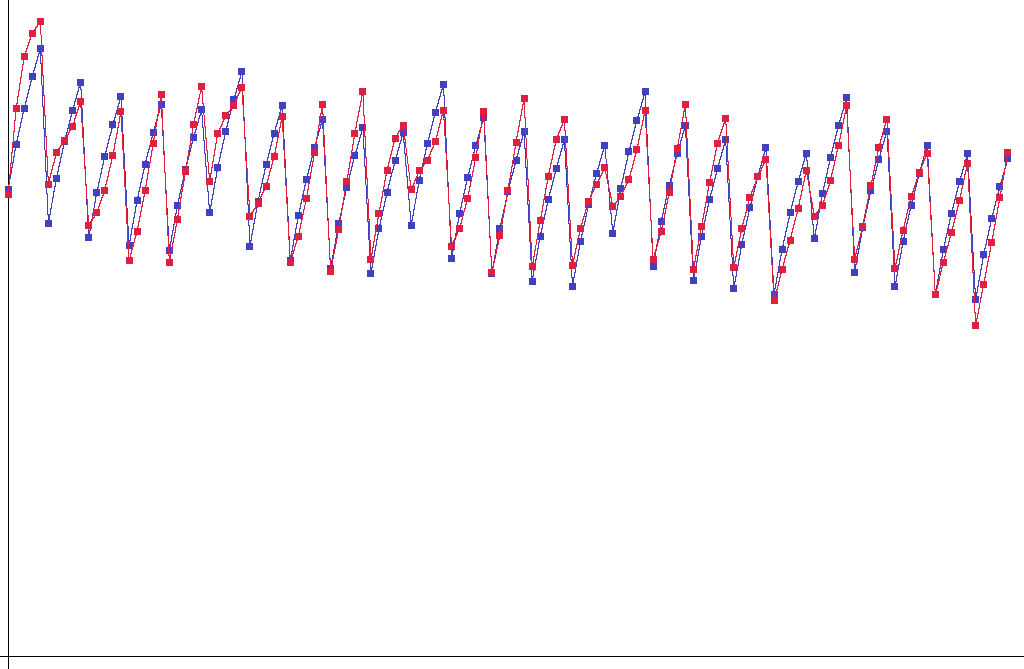
\includegraphics[scale=0.7]{livro}
		\end{center}

\vspace{100mm}

Teste 4.1 | Comando lista | Caos

lista

1 2 -1 2

0.1

3 4 500

782 395

0.24646 0.36143 0.65857 1.20000 [...]

0.71073 [...]

0.94663 0.96502 0.68823 0.42696 [...]

1.03693 [...]

Average Error 1.672466869627653\%

alfa = 0.10002900000000003

Gr\'afico:

		\begin{center}
		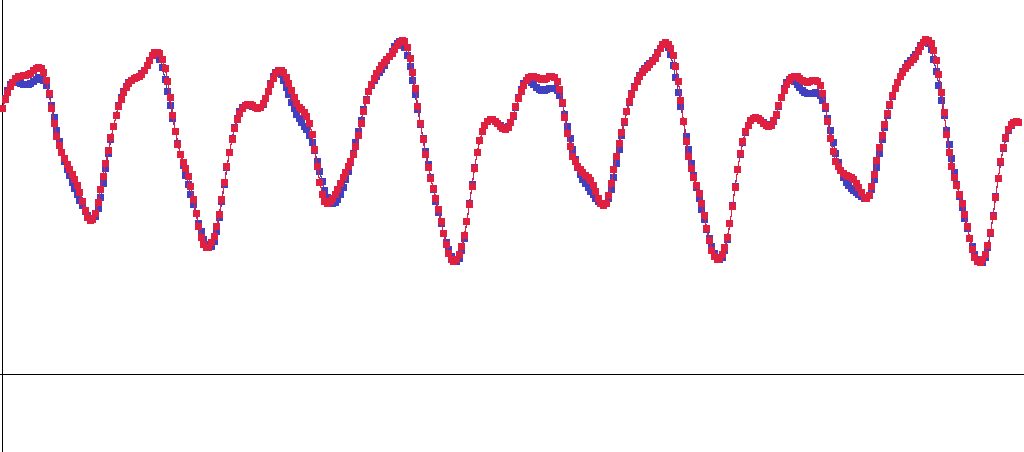
\includegraphics[scale=0.7]{lista}
		\end{center}

\vspace{100mm}

Teste 4.2 | Comando lista | 4 Retroalimenta\c{c}\~oes

lista

1 2 -1 2

0.1

3 4 500

782 395 4

0.24646 0.36143 0.65857 1.20000 [...]

0.71073 [...]

0.94663 0.96502 0.68823 0.42696 [...]

1.03693 [...]

Average Error 0.872818089005032\%

alfa = 0.1

Gr\'afico:

		\begin{center}
		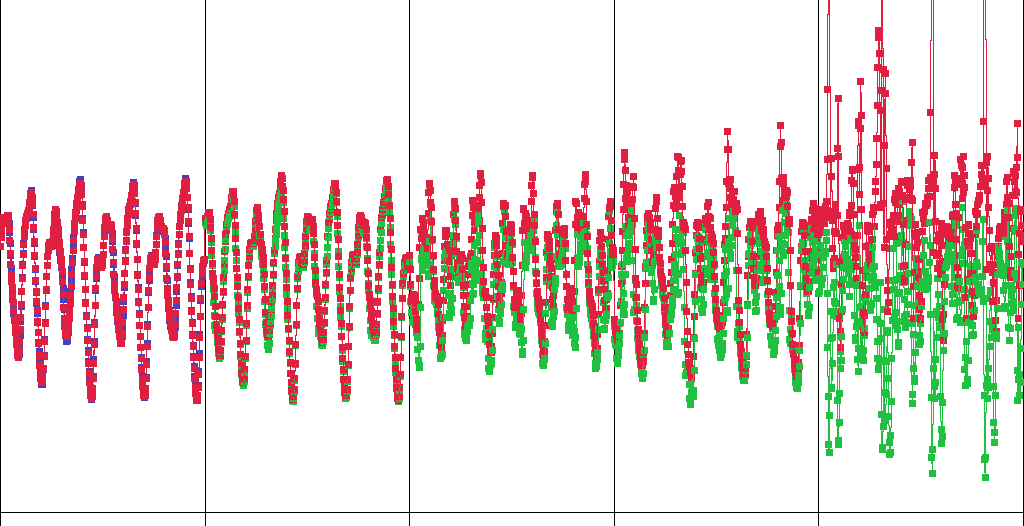
\includegraphics[scale=0.7]{retro}
		\end{center}

\vspace{100mm}

Teste Intervalar 1 | Caso Geral | Uma vari\'avel

curva

-6.4 6.4 -0.1 7.5

0.01 0.011

5 1 90

-6.3 -6.29 6.3 6.31 0.1

-6.3 -6.29 6.3 6.31 0.1

Average Error 8.109266994187609 \%

alfa = Interval [min=0.01, max=0.011]

		\begin{center}
		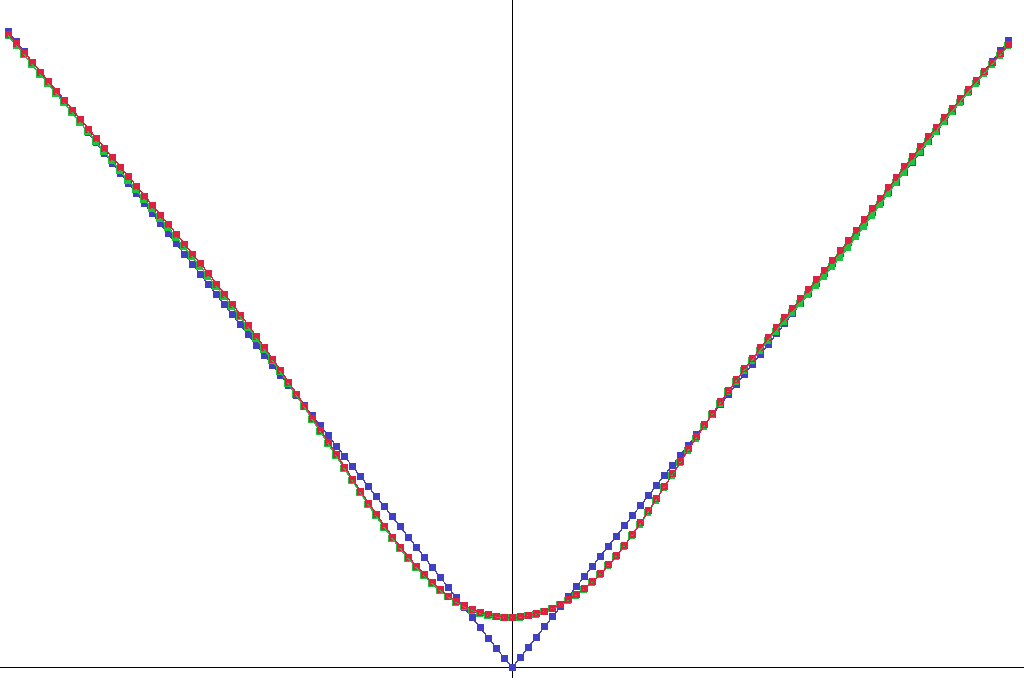
\includegraphics[scale=0.7]{intervalar1}
		\end{center}

\vspace{100mm}

Teste Intervalar 2 | Caso Geral | Duas vari\'aveis

curva

-6.4 6.4 -6.5 12.5

0.0001 0.000101

5 2 200

-6 -5.999999 6 6.000001 1

-5.5 -5.499999 5.5 5.500005 1

Average Error 141.02963794087555\%

alfa = Interval [min=1.0E-4, max=1.01E-4]

Gr\'afico:

		\begin{center}
		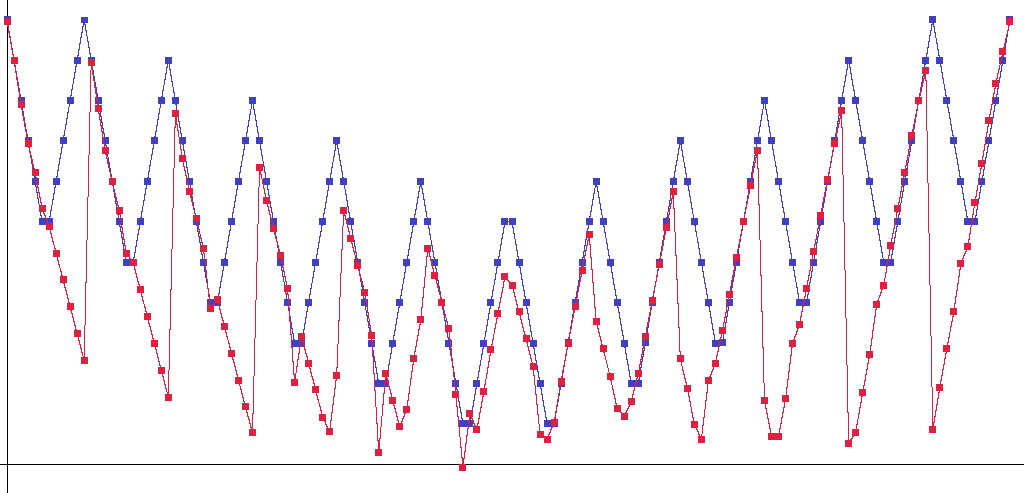
\includegraphics[scale=0.7]{intervalar2}
		\end{center}

\vspace{150mm}

Teste Intervalar 3 | Comando livro | Tr\^es vari\'aveis

livro

-1 126 -0.1 8

0.0001 0.000101

3 3 50

1 1.1 6 6.1 1

1.5 1.6 5.5 5.6 1

Average Error 17.87666281199084 \%

alfa = Interval [min=1.0E-4, max=1.01E-4]

Gr\'afico:

		\begin{center}
		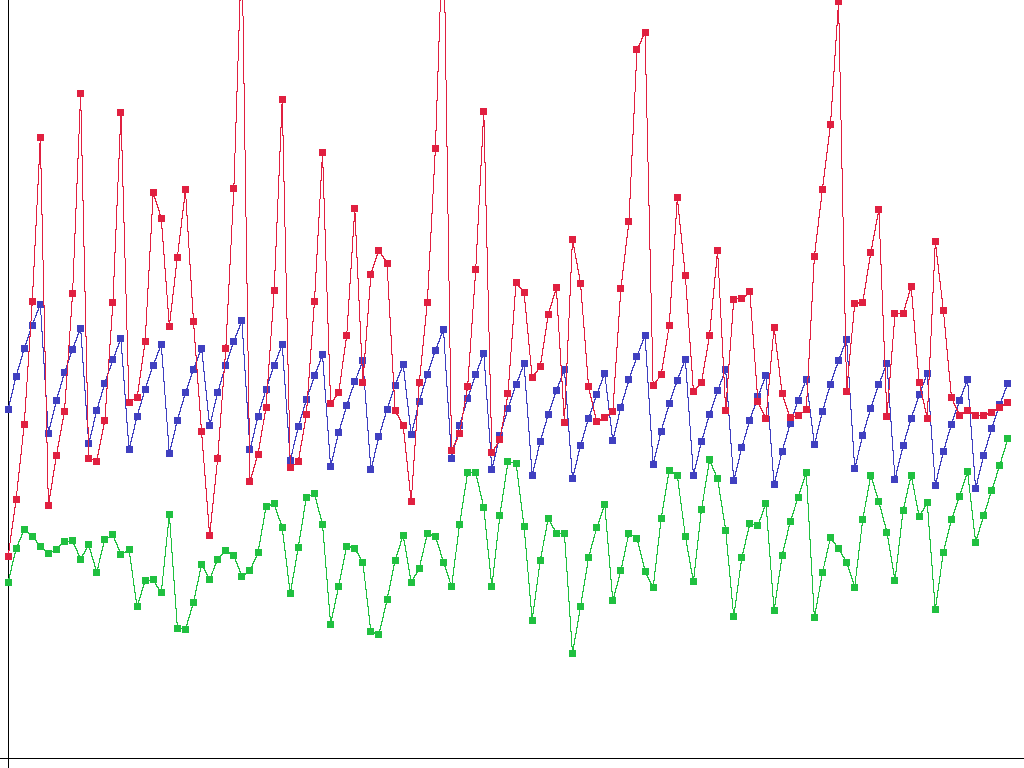
\includegraphics[scale=0.7]{intervalar3}
		\end{center}

\vspace{3mm}

Fa\c{c}a o download dos fontes e confira via este link: \href{http://spiritistwiki.herokuapp.com/spiritistwiki.zip}{\color{blue}\underline{spiritistwiki}}

\vspace{3mm}

Fora da caridade, n\~ao h\'a salva\c{c}\~ao. Com caridade, h\'a evolu\c{c}\~ao.

Vinicius Claudino Ferraz, Vers\~ao $1$ de 20/Abril/2020

\end{document}
